\documentclass{article}

\usepackage{verbatim}
\usepackage{amsmath,amsfonts}
\usepackage{enumerate}
\usepackage{fancyvrb}
\usepackage{graphicx}
\usepackage{fullpage}

\newcommand{\ds}{\ensuremath{\displaystyle}}
\newcommand{\floor}[1]{\ensuremath{\left\lfloor#1\right\rfloor}}
\newcommand{\fracpart}[1]{\ensuremath{\left\{#1\right\}}}

\title{Intermediate Test 4 -- Solutions}
\author{Stellenbosch Camp 2018}
\date{\vspace{-12pt}}


\begin{document}

\maketitle

\begin{enumerate}[1.]

\item % The Phil
\textit{How many numbers from $1$ to $2018$ inclusive can be written as the difference of two perfect squares?}

We say that a number is \emph{nice} if it can be written as the difference of two perfect squares. Any odd number is nice, since $2k+1 = (k+1)^2 -k^2$. Also, any number divisible by $4$ is nice since $4k = (k+1)^2 -(k-1)^2$. So looking at remainders modulo $4$, any number with remainder $0$, $1$ or $3$ is nice; on the other hand, since all perfect squares have remainder $0$ or $1$ modulo 4, the only possibilities for the remainder of a difference of two squares are $0$, $3$ and $1$; hence the numbers with these remainders are precisely the nice numbers.

So to count the nice numbers from $1$ to $2018$, we take the total amount of numbers ($2018$) and subtract those with remainder $2$; since $2018$ has a remainder of $2$ modulo $4$, the amount of the latter is $\floor{\frac{2018}{4}} +1$, yielding a final answer of \[ 2018 - \floor{\frac{2018}{4}} -1 = 1513. \]


\vspace{12pt}
\item %
\textit{Solve for lengths $x$ and $y$ in the following diagram:}

\begin{figure}[h]
\centering
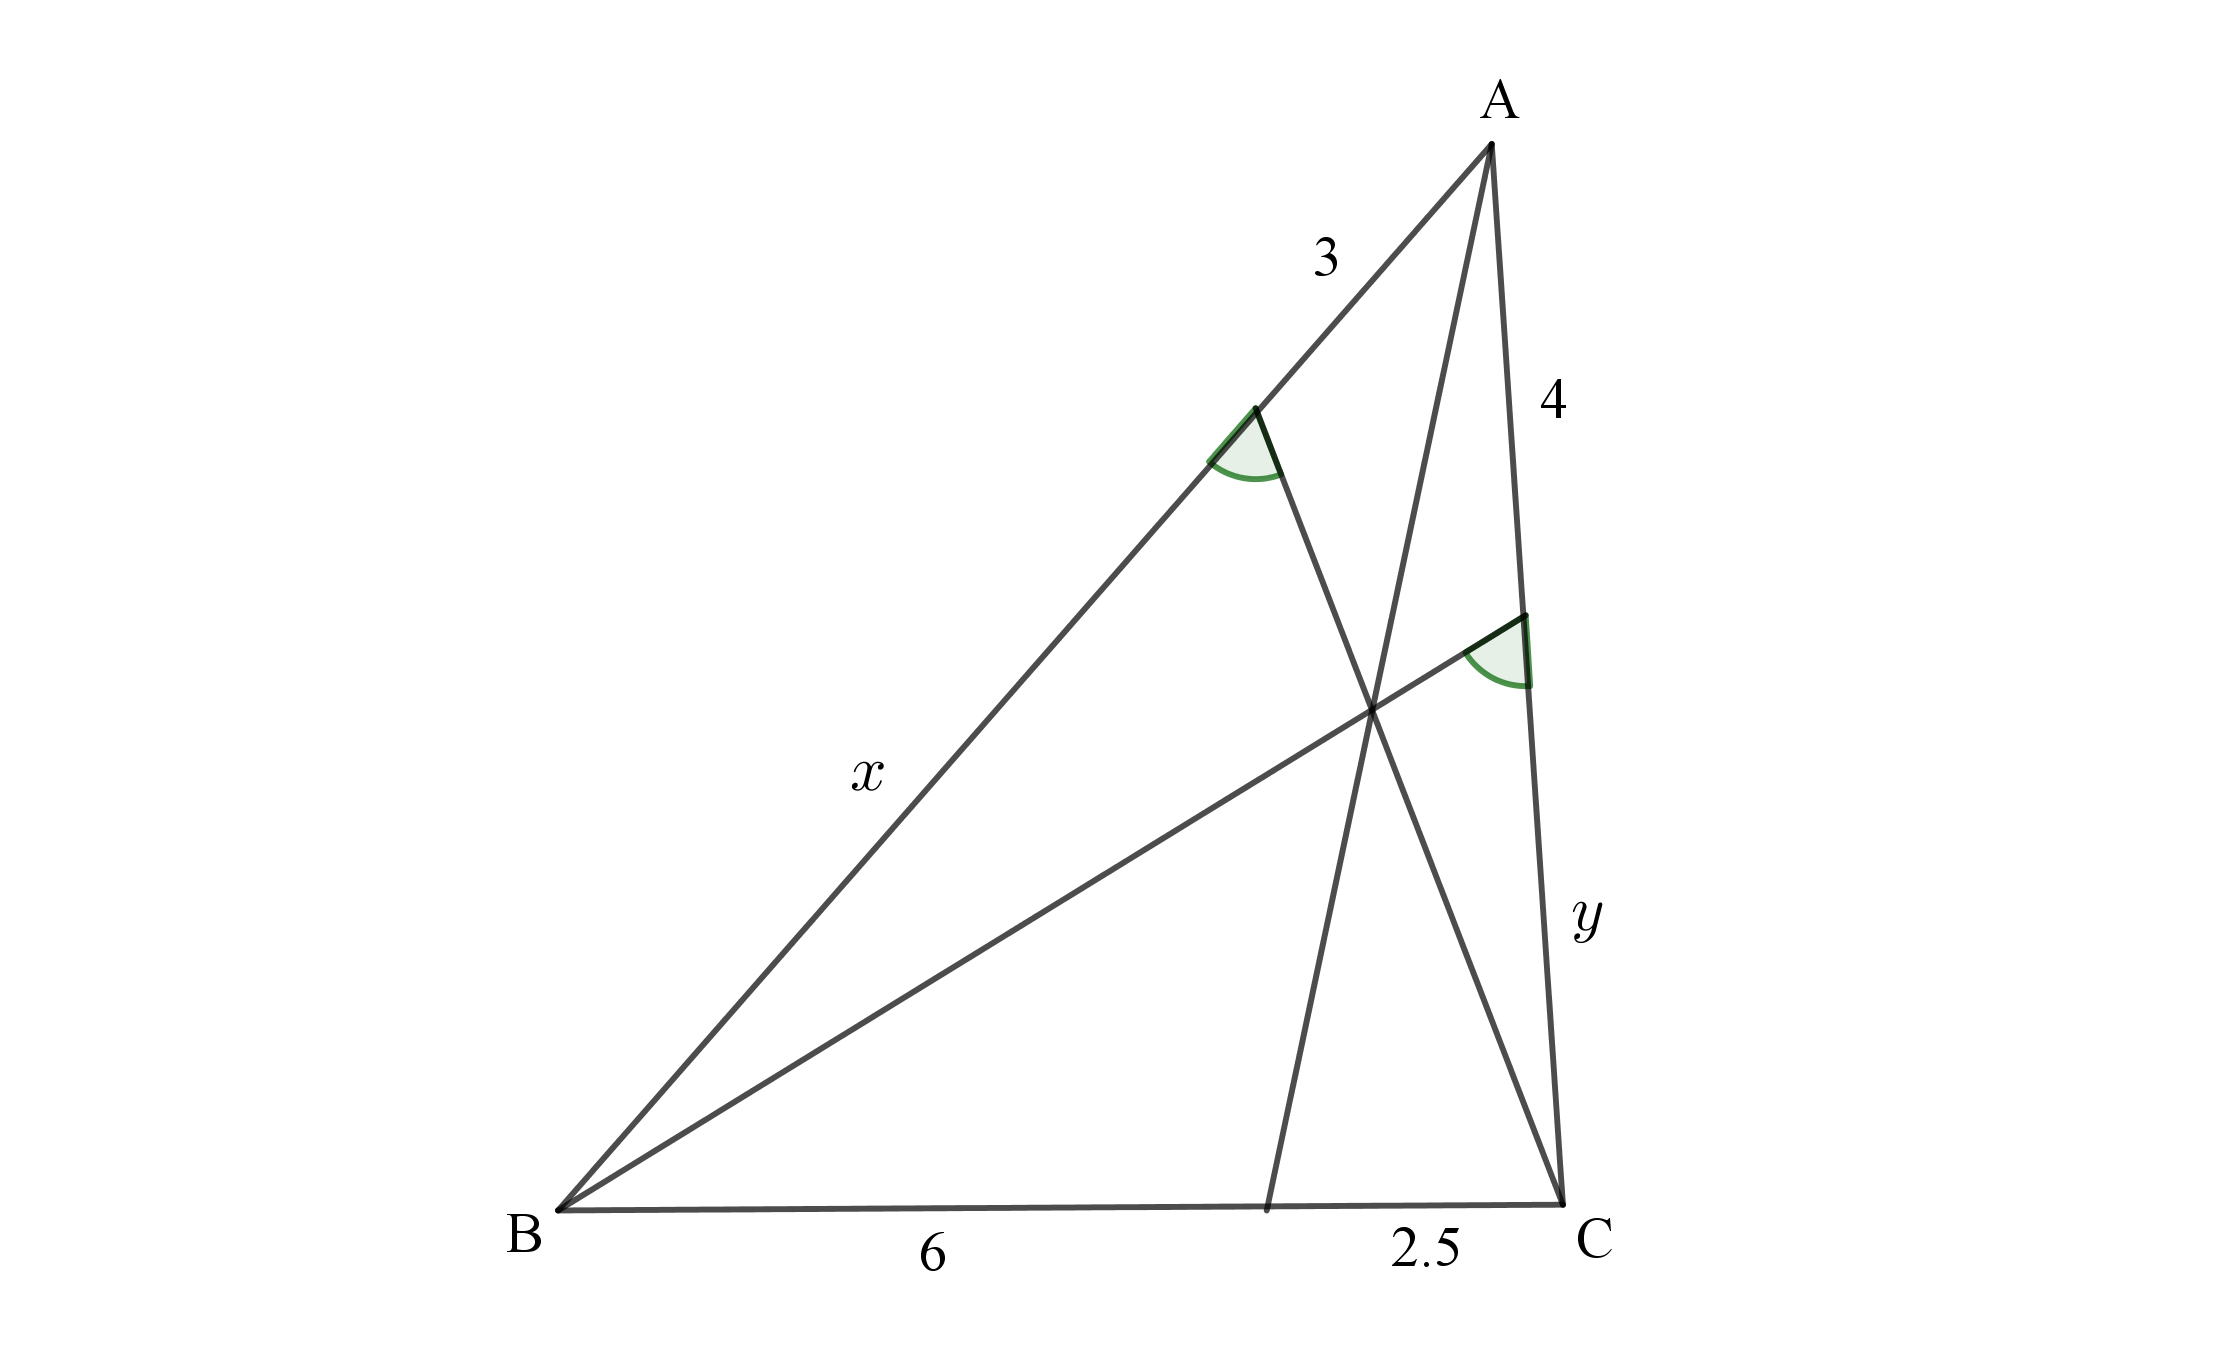
\includegraphics[width=0.6\textwidth]{GeogebraTest4.png}
\end{figure}


\vspace{6pt}
\item % The Dylan
\textit{Find all functions $f : \mathbb{R} -> \mathbb{R}$ such that for all real numbers $x$, \[ 2 f(x) +3 f(1-x) = x-4x^3. \]}


\vspace{6pt}
\item % AoPS:  https://artofproblemsolving.com/community/c6t309f6h455752_integers_in_infinite_chessboard
\textit{Prove that it is impossible to write a positive integer in every cell of an infinite chessboard, in such a manner that, for all positive integers $m, n$, the sum of numbers in every $m\times n$ rectangle is divisible by $m + n$.}


\vspace{12pt}
\item % Estonia 2007
\textit{An exam with $k$ questions is presented to $n$ students. A student fails the exam if they get less than half the answers right. We say that a question is easy if more than half of the students get it right. Decide if it is possible that}

\vspace{-12pt}
\textit{
\begin{enumerate}
  \item[(a)]  All students fail even though all the questions were easy.
  \item[(b)] No student fails even though no question was easy.
\end{enumerate}
}

\end{enumerate}


\vfill
\centering
\begin{BVerbatim}
 ,    /-.
((___/ __>
/      }
\ .--.(    ___
 \\   \\  /___\
\end{BVerbatim}

\end{document}
